\section{HÀM SỐ VÀ ĐỒ THỊ}
\subsection{TÓM TẮT LÝ THUYẾT}
\subsubsection{Khái niệm hàm số. Tập xác định và tập giá trị của hàm số}
\begin{itemize}
	\item [\iconMT] \indam{ĐỊnh nghĩa:} Giả sử $x$ và $y$ là hai đại lượng biến thiên và $x$ nhận giá trị thuộc tập số $\mathscr{D}$.	Nếu với \indamm{mỗi giá trị $x$ thuộc $\mathscr{D}$}, ta xác định được \indamm{một và chỉ một giá trị tương ứng $y$} thuộc tập hợp số thực $\mathbb{R}$ thì ta có một hàm số.
	\begin{boxkn}
		\begin{itemize}
			\item Ta gọi $x$ là biến số và $y$ là hàm số của $x$.
			\item Tập hợp $\mathscr{D}$ được gọi là tập xác định của hàm số.
			\item Tập hợp $T$ gồm tất cả các giá trị $y$ (tương ứng với $x$ thuộc $\mathscr{D}$) gọi là tập giá trị của hàm số.
		\end{itemize}
	\end{boxkn}
	\item [\iconMT] \indam{Cách cho một hàm số:} Một hàm số có thể được cho bởi một công thức hoặc nhiều công thức; có thể cho bằng mô tả; cho bằng bảng hoặc cho bằng biểu đồ.
\end{itemize}
\begin{vidu}
	Bản tin dự báo thời tiết cho biết nhiệt độ ở một số thời điểm trong ngày 01/05/2021 tại thành phố Hồ Chí Minh được ghi lại với biểu đồ bên dưới\\
	\centerline{\begin{tikzpicture}[font=\footnotesize, x=1.2cm,line join=round, line cap=round, >=stealth,scale=0.7,color=cyan]
		\draw[->] (.5,0)--(.5,5.5)node[left]{nhiệt độ};
		\draw[->] (.5,0)--(9,0) node[below]{giờ};
		\foreach \x/\y in {0/24,1/26,2/28,3/30,4/32,5/34} {
			\draw (.5,\x) node[left]{$\y$};}
		\foreach \x/\y in {1/1,2/4,3/7,4/10,5/13,6/16,7/19,8/22}\draw (\x,0.1)--(\x,-0.1) node [below] {\footnotesize $\y$};
		\foreach \x in {1,2,...,5} { \draw[orange!30] (.5,\x)--(9,\x); }
		\draw [line width=1pt,blue] (1,2)node[above]{\scriptsize $28$}--(2,1.5)node[above]{\scriptsize $27$}--(3,2)node[above left]{\scriptsize $28$}--(4,4)node[above]{\scriptsize $32$}--(5,3.5)node[above]{\scriptsize $31$}--(6,2.5)node[above]{\scriptsize $29$}--(7,2)node[above]{\scriptsize $28$}--(8,1.5)node[above]{\scriptsize $27$};
	\end{tikzpicture}}\\
Rõ ràng với mỗi mốc giờ xác định trong ngày, ta có tương ứng duy nhất 1 số đo nhiệt độ được dự báo nên  có xem đây là 1 hàm số với
	\begin{itemize}
		\item  Tập xác định $D=\{1;4;7;10;13;16;19;22\}$
		\item  Tập giá trị $T=\{28; 27; 32;31;29\}$.
	\end{itemize}
\end{vidu}
\begin{vidu}
	Xét công thức $y=2x+1$. Ta đã biết đây là một hàm số bậc nhất với
	\begin{itemize}
		\item  Tập xác định $D=\mathbb{R}$
		\item  Tập giá trị $T=\mathbb{R}$.
	\end{itemize}
\end{vidu}
\subsubsection{Đồ thị hàm số}
\begin{itemize}
	\item [\iconMT] \indam{Định nghĩa:} Cho hàm số $y=f(x)$ có tập xác định $\mathscr{D}$. Trên mặt phẳng toạ độ $Oxy$, đồ thị $(C)$ của hàm số là tập hợp tất cả các điểm $M(x;y)$ với $x \in \mathscr{D}$ và $y=f(x)$. Vậy $(C)=\{M(x;f(x)) \mid x \in \mathscr{D}\}$.
	\item [\iconMT] \indam{Lưu ý:} Điểm $M\left(x_{M};y_{M}\right)$ thuộc đồ thị hàm số $y=f(x)$ khi và chỉ khi $x_{M} \in \mathscr{D}$ và $y_{M}=f\left(x_{M}\right)$.
\end{itemize}
\subsubsection{Sự đồng biến, hàm số nghịch biến của hàm số}
\begin{itemize}
	\item [\iconMT] \indam{Khái niệm:} Với hàm số $y=f(x)$ xác định trên khoảng $(a;b)$, ta nói
	\begin{itemize}
		\item [\iconCH] Hàm số đồng biến trên khoảng $(a;b)$ nếu
		\boxmini{$\forall x_{1}, x_{2} \in(a ; b), x_{1}<x_{2} \Rightarrow f\left(x_{1}\right)<f\left(x_{2}\right)$}
		\item [\iconCH] Hàm số nghịch biến trên khoảng $(a;b)$ nếu
		\boxmini{$\forall x_{1}, x_{2} \in(a ; b), x_{1}<x_{2} \Rightarrow f\left(x_{1}\right)>f\left(x_{2}\right)$}
	\end{itemize}
	\item [\iconMT] \indam{Lưu ý:} Khi vẽ bảng biến thiên, xét từ trái sang phải, ta dùng mũi tên đi xuống để minh họa khoảng nghịch biến và mũi tên đi lên để minh họa khoảng đồng biến. 
\end{itemize}

\subsection{RÈN LUYỆN KĨ NĂNG GIẢI TOÁN}
\begin{dang}{Tính giá trị của hàm số tại một điểm}
	Cho hàm số $y=f(x)$ có tập xác định $\mathscr{D}$ và $x_0 \in \mathscr{D}$.
	\begin{itemize}
		\item[\faPencilSquareO] Tính giá trị hàm số tại $x_0$: Ta chỉ việc thay $x_0$ vào biểu thức $y=f(x)$, tìm được $y_0$.
		\item[\faPencilSquareO] Nếu $f(x)$ là hàm cho bởi nhiều biểu thức thì ta thay $x_0$ vào biểu thức mà miền xác định của nó chứa $x_0$.
	\end{itemize}
\end{dang}

\begin{vd}
	Cho hai hàm số $f(x)=x^2-2x$ và $g(x)=1-x$. Tính $f(1)$; $g(-2)$; $f(1)+g(-2)$.
\end{vd}

\dongcham{7}
\begin{vd}
	Cho hàm số $f(x)=\heva{&3x-2 &\text{với } &x\ge 1 \\&1-2x^2 &\text{với } &x<1}$. Tính $f(1), f(2), f(0), f(-3)$.
\end{vd}
\dongcham{5}


\begin{vd}
	Cho hàm số $y=2x^3-3(m-1)x+2$, với $m$ là tham số. 
	\begin{tasks}
		\task Tìm $m$ để đồ thị hàm số đi qua điểm $M(1;2)$.
		\task Tìm $m$ để đồ thị hàm số đi qua điểm $N(-3;1)$.
	\end{tasks}
\end{vd}
\dongcham{5}
\begin{vd}
\immini{ Cho hàm số $y=f(x)$ và hàm số $y=g(x)$ có đồ thị như hình bên.
	\begin{tasks}
		\task Trong các điểm $A(2;2)$ $B(4;2)$, $C(3;3)$ điểm nào thuộc đồ thị $f(x)$? điểm nào thuộc đồ thị $g(x)$?
		\task Tính giá trị $f(1)+g(2)$.
		\task Tìm điểm trên đồ thị $f(x)$ có tung độ bằng $3$.
	\end{tasks}
}{
	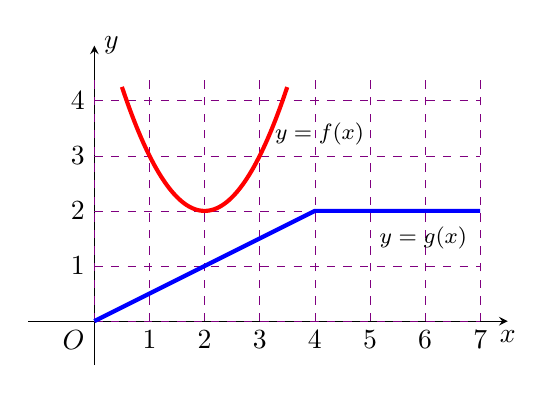
\begin{tikzpicture}[>=stealth,scale=0.7]
	\draw[->] (-1.2,0)--(0,0)%
	node[below left]{$O$}--(7.5,0) node[below]{$x$};
	\draw[->] (0,-0.8) --(0,5) node[right]{$y$};
	\foreach \x in {1,2,3,4,5,6,7}{
		\draw (\x,0) node[below]{$\x$};%Ox
	}
	\foreach \y in {1,2,3,4}{
		\draw (0,\y) node[left]{$\y$};%Oy
	}
	\draw[violet,dashed,line width=0.2pt] (0,0) grid (7,4.5);
	\draw [blue, line width=1.5pt] (0,0)--(4,2)--(7,2);
	\draw [red, line width=1.5pt, domain=0.5:3.5, samples=100] %
	plot (\x, {(\x)^2 -4*(\x)+6});
	\draw (3.1,3.4)node[right]{\footnotesize$y=f(x)$} (5,1.5)node[right]{\footnotesize $y=g(x)$};
	
	\end{tikzpicture}}
\end{vd}
\dongcham{7}
\begin{dang}{Tìm tập xác định, tập giá trị của hàm số}
	\begin{itemize}
		\item [\iconMT] \indam{Tập xác định:} Ta tìm tập hợp tất cả các giá trị của $x$ để hàm số đã cho có nghĩa. Cần lưu ý hai vấn đề sau:
		\begin{listEX}[2]
			\item [\ding{172}] $\dfrac{A}{B}$ có nghĩa khi $B \ne 0$.
			\item [\ding{173}] $\sqrt{B}$ có nghĩa khi $B \ge 0$.
		\end{listEX}
		\item [\iconMT] \indam{Tập giá trị:} Với $x$ thuộc miền xác định $\mathscr{D}$, ta có thể căn cứ vào bảng biến thiên hoặc đồ thị để tìm miền giá trị (\textit{nhìn khoảng "dao động" của} $y$.).
	\end{itemize}

\end{dang}

\begin{vd}%[0D2B1-1]
	Sau khi đun nóng băng phiến lên đến gần $90^{\circ}C$, người ta để nguội, quan sát, ghi nhận nhiệt độ và trạng thái của băng phiến sau mẫu phút như bảng sau
	\begin{center}
	\textit{Nhiệt độ và trạng thái của băng phiến khi để nguội}
		\begin{tabular}{|l|c|c|c|c|c|c|c|c|c|c|c|}
			\hline 
			\textbf{Thời gian nguội (phút)} & $0$ & $1$ & $2$ & $3$ & $4$ & $5$ & $6$ & $7$ & $8$ & $9$ & $10$ \\ 
			\hline 
			\textbf{Nhiệt độ ($^{\circ}C$)} & $86$ & $84$ & $82$ & $81$ & $80$ & $80$ & $80$  &$80$ & $79$ & $77$ & $75$ \\
			\hline
			\textbf{Trạng thái} & \multicolumn{4}{|c|}{lỏng} &\multicolumn{4}{|c|}{lỏng và rắng} & \multicolumn{3}{|c|}{rắn}\\
			\hline
		\end{tabular}
	\end{center}
\begin{tasks}(1)
	\task Tại sao từ bảng trên, có thể nói nhiệt độ của băng phiến là một hàm số theo thời gian (nung nóng)? Tìm tập xác định và tập giá trị của hàm số trên.
	\task Sau khi để nguội $3$ phút, nhiệt độ băng phiến là bao nhiêu?
	\task Băng phiến chuyển hoàn toàn sang trạng thái rắn sau bao nhiêu phút?
\end{tasks}
	\loigiai{
		\begin{enumerate}[a)]
			\item Bảng giá trị cho thấy nhiệt độ (kí hiệu là $y$) là một hàm số theo thời gian (kí hiệu là $x$) vì khi cho $x$ một giá trị bất kì, ta luôn tìm được duy nhất một giá trị của $y$. Do vậy bảng này xác định một hàm số biểu thị nhiệt độ của băng phiến theo thời gian.\\
			Từ bảng giá trị của hàm số, ta có tập xác định $\mathscr{D}=\{0 ; 1 ; 2 ; 3 ; 4 ; 5 ; 6 ; 7 ; 8 ; 9 ; 10\}$ và tập giá trị $T=\{75 ; 77 ; 79 ; 80 ; 81 ; 82 ; 84 ; 86\}$.
			\item Sau khi để nguội $3$ phút, nhiệt độ băng phiến là $81^{\circ}C$.
			\item Băng phiến chuyển hoàn toàn sang trạng thái rắn sau $8$ phút (lúc đó nhiệt độ băng phiến là $79^{\circ}$).
		\end{enumerate}
	}
\end{vd}
\dongcham{5}
\begin{vd}
	\immini{Cho hàm số $y=f(x)$ có tập xác định là $\mathscr{D}$ và đồ thị là đường liền nét được vẽ trên miền $\mathscr{D}$ như hình bên
	\begin{tasks}(1)
		\task Xác định tập xác định $\mathscr{D}$.
		\task Tìm tập giá trị của hàm số trên miền $\mathscr{D}$.
		\task Tìm các điểm thuộc đồ thị và có tung độ bằng $3$.
	\end{tasks}}{
	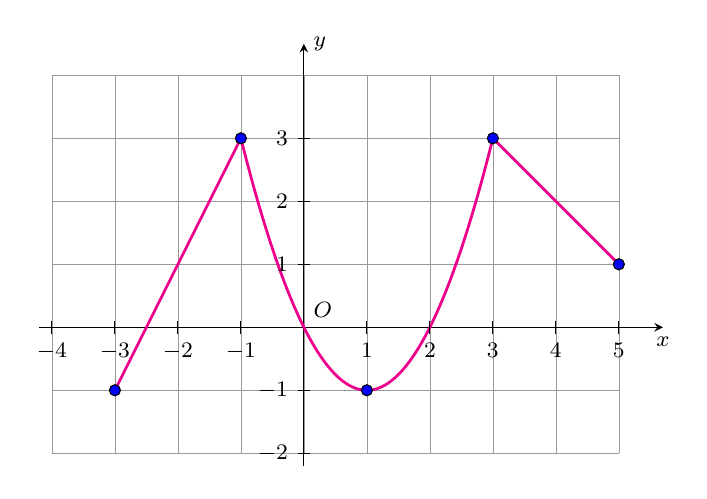
\begin{tikzpicture}[smooth,samples=300,scale=0.8,>=stealth,font=\footnotesize]
		\draw[line width=0.1pt,gray!80] (-4,-2) grid (5,4);
		\draw[->] (-4.2,0)--(5.7,0) node[below]{$x$};
		\draw[->] (0,-2.2)--(0,4.5) node[right]{$y$};
		\draw (0,0) node[above right]{$O$};
		\draw[line width=1pt,domain=-1:3,magenta] plot(\x,{(\x-1)^2-1});
		\draw[line width=1pt,magenta] (-3,-1)--(-1,3) (3,3)--(5,1);
		\draw[fill=blue] (-3,-1) circle(2.5pt) (-1,3) circle(2.5pt) (3,3) circle(2.5pt) (5,1) circle(2.5pt) (1,-1) circle(2.5pt);
		\foreach \x in {-4,-3,-2,-1,1,2,3,4,5}\draw (\x,0.1)--(\x,-0.1) node [below] {\footnotesize $\x$};
		\foreach \y in {-2,-1,1,2,3}\draw (0.1,\y)--(-0.1,\y) node [left] {\footnotesize $\y$};
\end{tikzpicture}}
\end{vd}
\dongcham{5}
\begin{vd}
	Tìm tập xác định của các hàm số sau đây:
	\begin{listEX}[2]
		\item $y=x^4+x^2-2$.
		\item $y=\dfrac{x+2}{x-2}$.
		\item $y=\dfrac{x^2+2}{4-x}$.
		\item $y=\dfrac{1}{-x^2+3x}$
	\end{listEX}
\end{vd}
\dongcham{12}
\begin{vd}
	Tìm tập xác định của các hàm số sau đây:
	\begin{listEX}[2]
		\item $y=\sqrt{x-2}$.
		\item $y=\dfrac{2x-1}{\sqrt{x+2}}$.
		\item $y=x+\dfrac{1}{\sqrt{3-x}}$.
		\item $y=\sqrt{2+x}+\sqrt{x-2}$.
	\end{listEX}
\end{vd}
\dongcham{12}
\begin{vd}
	Tìm tập xác định của các hàm số sau:
	\begin{listEX}[2]
		\item $f(x)=\heva{&2x+1 &\text{ nếu }& x \le 0 \\& x^2 &\text{ nếu }& x > 0}$.
		\item $f(x)=\heva{&\dfrac{1}{x-1}&\text{ nếu }& x \le 2 \\& x^2 &\text{ nếu }& x > 2}$.
	\end{listEX}
\loigiai{
	\begin{enumerate}[a)]
		\item Ta xét hai trường hợp
		\begin{itemize}
			\item [$\bullet$] Khi $x\le 0$ thì $f(x)=2x+1$. Hàm này luôn xác định với mọi $x \in \mathbb{R}$ nên sẽ xác định với mọi $x \le 0$.
			\item [$\bullet$] Khi $x>0$ thì $f(x)=x^2$. Hàm này luôn xác định với mọi $x\in \mathbb{R}$ nên sẽ xác định với mọi $x >0$.
		\end{itemize}
	Kết hợp hai trường hợp, ta được tập xác định của hàm số là $\mathscr{D}=\mathbb{R}$.
		\item Ta xét hai trường hợp
		\begin{itemize}
			\item [$\bullet$] Khi $x\le 2$ thì $f(x)=\dfrac{1}{x-1}$. Hàm này  xác định khi và chỉ khi $x-1 \ne 0 \Leftrightarrow x \ne 1$.
			\item [$\bullet$] Khi $x>2$ thì $f(x)=x^2$. Hàm này luôn xác định với mọi $x\in \mathbb{R}$ nên sẽ xác định với mọi $x >2$.
		\end{itemize}
		Kết hợp hai trường hợp, ta được tập xác định của hàm số là $\mathscr{D}=\mathbb{R}\backslash \{1\}$.
\end{enumerate}}
\end{vd}
\dongcham{10}

\begin{dang}{Tìm khoảng đồng biến, khoảng nghịch biến của hàm số}
\begin{itemize}
	\item[\faPencilSquareO] Nếu đề bài cho bảng biến thiên hoặc đồ thị: Xét từ trái sang phải thì
	\begin{itemize}
		\item [$\bullet$] Khoảng nào có mũi tên đi xuống (đồ thị đổ xuống) thì khoảng đó hàm số nghịch biến.
		\item [$\bullet$] Khoảng nào có mũi tên đi lên (đồ thị đi lên) thì khoảng đó hàm số đồng biến.
	\end{itemize}
	\item[\faPencilSquareO] Nếu đề bài yêu cầu xét tính đồng biến, nghịch biến của hàm số $y=f(x)$ trên khoảng xác định $(a;b)$:  Ta lấy $x_1, x_2$ tùy ý thuộc $(a;b)$, với $x_1<x_2$ và tính $f(x_1)-f(x_2)$, nếu
	\begin{itemize}
		\item [$\bullet$] $f(x_1)-f(x_2)<0$ thì hàm số $y=f(x)$ đồng biến trên khoảng $(a;b)$.
		\item [$\bullet$] $f(x_1)-f(x_2)>0$ thì hàm số $y=f(x)$ nghịch biến trên khoảng $(a;b)$.
	\end{itemize}
	\item[\faPencilSquareO] Trong nhiều trường hợp, để tìm được khoảng đồng biến và nghịch biến của hàm số, ta có thể lập bảng biến thiên của hàm số đó trên miền xác định.
\end{itemize}
\end{dang}
\begin{vd}
	\immini{Cho hàm số $y=f(x)$ có tập xác định là $\mathscr{D}$ và đồ thị là đường liền nét được vẽ trên miền $\mathscr{D}$ như hình bên. Tìm các khoảng đồng biến và nghịch biến của hàm số trên miền $\mathscr{D}$.
	}{
		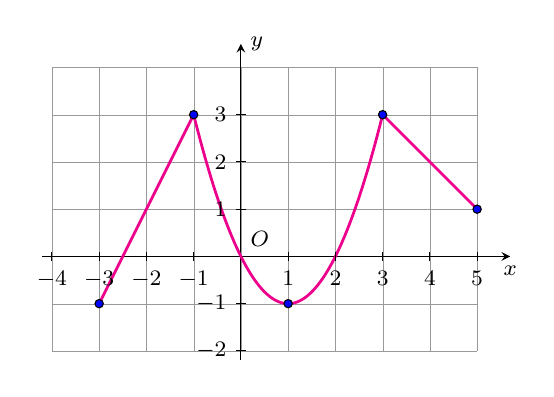
\begin{tikzpicture}[smooth,samples=300,scale=0.6,>=stealth,font=\footnotesize]
			\draw[line width=0.1pt,gray!80] (-4,-2) grid (5,4);
			\draw[->] (-4.2,0)--(5.7,0) node[below]{$x$};
			\draw[->] (0,-2.2)--(0,4.5) node[right]{$y$};
			\draw (0,0) node[above right]{$O$};
			\draw[line width=1pt,domain=-1:3,magenta] plot(\x,{(\x-1)^2-1});
			\draw[line width=1pt,magenta] (-3,-1)--(-1,3) (3,3)--(5,1);
			\draw[fill=blue] (-3,-1) circle(2.5pt) (-1,3) circle(2.5pt) (3,3) circle(2.5pt) (5,1) circle(2.5pt) (1,-1) circle(2.5pt);
			\foreach \x in {-4,-3,-2,-1,1,2,3,4,5}\draw (\x,0.1)--(\x,-0.1) node [below] {\footnotesize $\x$};
			\foreach \y in {-2,-1,1,2,3}\draw (0.1,\y)--(-0.1,\y) node [left] {\footnotesize $\y$};
	\end{tikzpicture}}
\end{vd}
\dongcham{1}
\begin{vd}
	Cho hàm số $y=f(x)=-2x^2-7$. Xét tính đồng biến và nghịch biến của hàm số trên các khoảng $(-4;0)$; $(3;10)$.
\end{vd}

\dongcham{7}
\begin{vd}
	Xét tính đồng biến và nghịch biến của hàm số $y=f(x)=x^2+10x+9$ trên $(-5;+\infty)$.
\end{vd}
\dongcham{8}
\begin{vd}
	Xét tính đồng biến và nghịch biến của hàm số $y=f(x)=\dfrac{x}{x-7}$ trên các khoảng $(-\infty;7)$;  $(7;+\infty)$.
\end{vd}
\dongcham{10}
\begin{dang}{Vẽ đồ thị hàm số cho bởi nhiều biểu thức}
	
\end{dang}
\begin{vd}
	Tìm tập xác định và vẽ đồ thị các hàm số sau:
	\begin{tasks}(2)
		\task $f(x)=\heva{& 2x & \text{ với }& x \ge 0 \\ & -x & \text{ với }& x<0.}$
		\task $f(x)=\heva{& -x^2 & \text{ với }& x\le 1\\ & 1 & \text{ với }& x>1.}$
		\task $f(x)= \big|x\big|$.
		\task $f(x)= \big|x+2\big|$.
	\end{tasks}
\end{vd}

\dongcham{21}
\begin{dang}{Viết công thức hàm số cho một số bài toán thực tế}
\end{dang}

\begin{vd}%[0D2T1-1]
	Theo quyết định số 2019/QĐ-BĐVN ngày 01/11/2018 của Tổng công ty Bưu điện Việt Nam, giá cước dịch vụ Bưu chính phổ cập đối với dịch vụ thư cơ bản và bưu thiếp trong nước có khối lượng đến $250$g như trong bảng sau
	\immini{\begin{enumerate}[a)]
			\item Số tiền dịch vụ thư cơ bản phải trả $y$ (đồng) có là hàm số của khối lượng thư cơ bản $x$ (g) hay không? Nếu đúng, hãy xác định những công thức tính $y$.
			\item Tính số tiền phải trả khi bạn Dương gửi thư có khối lượng $150$g, $200$g.
	\end{enumerate} }
	{\vspace{0.6 cm}
		\begin{tabular}{|c|c|}
			\hline
			\textcolor{blue}{Khối lượng đến $250$ g} & \textcolor{blue}{Mức cước (đồng)}\\
			\hline
			Đến $20$ g & $4000$\\
			\hline
			Trên $20$ g đến $100$ g & $6000$ \\
			\hline
			Trên $100$ g đến $250$ g & $8000$\\
			\hline
	\end{tabular}}
	\loigiai{
		\begin{enumerate}[a)]
			\item Số tiền dịch vụ thư cơ bản phải trả $y$ là hàm số của $x$ vì mỗi giá trị của $x$ (chính là khối lượng của thư) có đúng một giá trị của $y$ (mức cước hay số tiền phải trả) tương ứng.\\
			Quan sát bảng ta thấy:
			\begin{itemize}
				\item[$\bullet$] Nếu khối lượng thư đến $20$ g hay $0<x \le 20$ thì mức cước phải trả là $4000$ đồng hay $y= 4000$.
				\item[$\bullet$] Nếu khối lượng thư trên $20$ g hay $100$ g hay $20 < x \le 100$ g thì mức cước là $6000$ đồng hay $y=6000$.
				\item[$\bullet$] Nếu khối lượng thư trên $100$ g đến $250$ g hay $100 < x \le 250$ thì mức cước là $8000$ đồng hay $y=8000$.
			\end{itemize}
			Vậy ta có công thức xác định $y$ như sau:
			$y=\heva{&4000&\text{nếu}& 0<x\le 20\\&6000&\text{nếu}& 20 <x\le 100\\&8000&\text{nếu}& 100<x\le 250.}$
			\item Vì $100 < 150 <250$ và $100 <200 <250$ nên bức thư có khối lượng $150$ g thì cần trả cước là $8000$ đồng và bức thư có khối lượng $200$ g cũng cần trả cước là $8000 $ đồng. \\
			Vậy tổng số tiền phải trả khi bạn Dương gửi thư có khối lượng $150$ g và $200$ g là \\ \centerline{$8000 + 8000 = 16 000$ (đồng).}
		\end{enumerate}
	}
\end{vd}
\dongcham{8}

\begin{vd}
	Nhiệt độ ở mặt đất đo được khoảng $30^{\circ} \mathrm{C}$. Biết rằng cứ lên $1 \mathrm{~km}$ thì nhiệt độ giảm đi $5^{\circ}$.
	\begin{tasks}(1)
		\task Hãy lập hàm số $T$ theo $h$, trong đó $T$ tính bằng độ $\left({ }^{\circ}\right)$ và $h$ tính bằng ki-lô-mét $(\mathrm{km})$.
		\task Hãy tính nhiệt độ khi ở độ cao $3 \mathrm{~km}$ so với mặt đất.
	\end{tasks}
	\loigiai{
		\begin{enumerate}[a)]
			\item Hàm số $T$ theo $h$ là $T=30-5h$.
			\item Thay $h=3$ vào công thức $T=30-5h$, ta được $
			T=30-5 \cdot 3=15$.\\
			Vậy khi lên độ cao $3 \mathrm{~km}$ thì nhiệt độ tại đó là $15^{\circ}$
	\end{enumerate}}
\end{vd}
\dongcham{8}
\begin{vd}%[0D2T1-1]
	Một công ty viễn thông A cung cấp dịch vụ truyền hình cáp với mức phí ban đầu là 300000 đồng và mỗi tháng phải đóng 150000 đồng. Công ty viễn thông B cũng cung cấp dịch vụ truyền hình cáp nhưng không tính phí ban đầu và mỗi tháng khách hàng sẽ phải đóng 200000 đồng.
	\begin{tasks}(1)
		\task Gọi $T$ (đồng) là số tiền khách hàng phải trả cho mỗi công ty viễn thông trong $t$ (tháng) sử dụng dịch vụ truyền hình cáp. Khi đó hãy lập hàm số $T$ theo $t$ đối với mỗi công ty.
		\task Tính số tiền khách hàng phải trả sau khi sử dụng dịch vụ truyền hình cáp trong 5 tháng đối với mỗi công ty.
		\task Khách hàng cần sử dụng dịch vụ truyền hình cáp trên mấy tháng thì đăng kí bên công ty viễn thông A sẽ tiết kiệm chi phí hơn?
	\end{tasks}
	\loigiai{
		\begin{enumerate}[a)]
			\item Hàm số $T$ theo $t$ đối với công ty A là $T=150000t+300000$.\\
			Hàm số $T$ theo $t$ đối với công ty B là $T=200000t$.
			\item Thay $t=5$ lần lượt vào hai công thức trên, ta được
			\begin{itemize}
				\item [$\bullet$] Số tiền phải trả trong 5 tháng khi sử dụng dịch vụ truyền hình cáp của công ty A là $150000.5+300000=1050000$ đồng.
				\item [$\bullet$] Số tiền phải trả trong 5 tháng khi sử dụng dịch vụ truyền hình cáp của công ty B là $200000.5=1000000$ đồng.
			\end{itemize}
			\item Để dịch vụ truyền hình cáp của công ty A lợi hơn dịch vụ truyền hình cáp của công ty B thì:
			$$
			150000t+300000<200000t \Leftrightarrow 300000<50000t \Leftrightarrow t>6
			$$
			Vậy nếu sử dụng từ 7 tháng trở lên thì sử dụng dịch vụ truyền hình cáp bên công ty A sẽ có lợi hơn.
	\end{enumerate}}
\end{vd}
\dongcham{16}
